%%% Demographic Research Pandoc Style
%%%
%%% Jonas Schöley
%%% jschoeley@gmail.com
%%%
%%% 2021-02-19
%%%
%%% Depends on file "drbibstyle.bst" for custom bibliography styling,
%%% "drtitling" for title formating,
%%% "drlogo.pdf" for the Demographic Research logo.
%%%
%%% Based upon the work of
%%% Jana Korsinek
%%% Peter Wilhelm
%%% Peter Wilson
%%% and very probably others such as the countless student assistants
%%% who, over the years, worked at Demographic Research.

%--- Documentclass -----------------------------------------------------

\documentclass[10pt,twoside,reqno]{article}
\raggedbottom

%--- Font/encoding -----------------------------------------------------

\usepackage[utf8]{inputenc} % .tex-file text encoding
\usepackage[T1]{fontenc}    % vector fonts and special chars in output
\usepackage{times}          % Times Roman font family

%--- Constants ---------------------------------------------------------

% provided by YAML header of markdown file

% document title
  \def \thetitle {The centered ternary balance scheme: A technique to
visualize surfaces of unbalanced three-part compositions}
  \def \theshorttitle {The centered ternary balance scheme}

% first page of document in volume
  \def \thestartpage {397}

% article and volume numbers
  \def \thearticle {17}
  \def \thevolume {44}

% date of publication
  \def \thedatepub {22 February 2021}

% category of article
  \def \thecat {Research Article}

% publication blurb
  \def \theblurb {This article is part of the Special Collection on
``Data Visualization,'' organized by Guest Editors Tim Riffe, Sebastian
Klüsener, and Nikola Sander.}

% author listings
  \def \theheadingauthor {Schöley}

% number of authors
\newcounter{authorcount}
   \stepcounter{authorcount} 

%--- Maths -------------------------------------------------------------

\usepackage{amsmath}  % various maths features
\usepackage{amssymb}  % maths symbols
\usepackage{mathrsfs} % maths script fonts

%--- Misc --------------------------------------------------------------

\usepackage{etoolbox} % allows to inject commands inside environments
\usepackage{placeins} % control the placement of floats via \FloatBarrier
\usepackage{xcolor}   % for colored links

%--- Figures -----------------------------------------------------------


  \usepackage{graphicx} % include external images

  % generate all images so they have a width \cnstmaxfigwidth
  % images get their normal width if they fit onto the page
  % images are scaled down if they would overflow the margins
  \makeatletter
    \def\cnstmaxfigwidth{
      \ifdim \Gin@nat@width>\linewidth
        \linewidth
      \else \Gin@nat@width
      \fi
    }
  \makeatother
  \let\Oldincludegraphics\includegraphics
  \renewcommand{\includegraphics}[1]{\Oldincludegraphics[width=\cnstmaxfigwidth]{#1}}

  \AfterEndEnvironment{figure}{\FloatBarrier}


%--- Captions ----------------------------------------------------------

% define caption style
\usepackage[hang]{caption}
\DeclareCaptionLabelSeparator{capsep}{:}
\DeclareCaptionFormat{capformat}{#1#2\hspace{1cm}#3}
\DeclareCaptionFont{capfont}{\normalsize\bfseries}
\captionsetup[figure]{
            style           = default,
            indention       = 2.4cm,
            labelsep        = capsep,
            format          = capformat,
            name            = Figure,
            font            = capfont,
            labelfont       = capfont,
            justification   = raggedright,
            singlelinecheck = false
}
\captionsetup[table]{
            style           = default,
            indention       = 2.25cm,
            labelsep        = capsep,
            format          = capformat,
            name            = Table,
            font            = capfont,
            labelfont       = capfont,
            justification   = raggedright,
            singlelinecheck = false
}

% captions above
\usepackage{float}
\floatstyle{plaintop}
\restylefloat{table}
\restylefloat{figure}

%--- Localization ------------------------------------------------------

% babel
\usepackage[english]{babel} % document language/localization
\usepackage{hyphenat}       % hyphenation rules

% hyphenation rules for specific words
  \hyphenation{}

%--- Links -------------------------------------------------------------

\usepackage{hyperref}
\hypersetup{
  hidelinks=true,
  breaklinks=true,
  colorlinks=false,
  pdftitle={\thetitle}
}
\urlstyle{rm}

%--- Bibliography ------------------------------------------------------

\usepackage{natbib}
\bibpunct [: ] {(} {)} {;} {a} {} {,}
\setcitestyle{aysep={}}
\bibliographystyle{drbibstyle}
% special doi and url format in bibliography (used in .bst file)
\newcommand{\doi}[1]{\href{https://www.dx.doi.org/#1}{\textcolor{blue}{doi:#1}}}
    % use url command to escape special chars in url
\newcommand{\biburl}[1]{\href{#1}{\textcolor{blue}{\url{#1}}}}
    % which url prefix to use
\newcommand{\urlprefix}{}

%--- General layout ----------------------------------------------------

% page layout
\usepackage{geometry}
\geometry{
  paperheight = 22cm,
  paperwidth  = 17cm,
  top         = 2.54cm,
  bottom      = 2.54cm,
  inner       = 2cm,
  outer       = 2.54cm,
  footskip    = 11mm,
  headheight  = 1cm,
  headsep     = 0.75cm,
  showframe   = false
}

% title and cover format
\usepackage{drtitling}

% spacing
\setlength{\parskip}{0ex}
\setlength{\parindent}{.7cm}
\setlength{\bibsep}{.18cm}
\setlength{\belowdisplayskip}{15pt} \setlength{\belowdisplayshortskip}{10pt}
\setlength{\abovedisplayskip}{15pt} \setlength{\abovedisplayshortskip}{10pt}

% avoid orphans and widows
\widowpenalty = 10000
\clubpenalty  = 10000

% don't break footnotes
\interfootnotelinepenalty = 10000

% don't hyphenate across pages
\brokenpenalty10000\relax

%--- Lists -------------------------------------------------------------

% tight lists
\providecommand{\tightlist}{%
  \setlength{\topsep}{0pt}
  \setlength{\partopsep}{0pt}
  \setlength{\itemsep}{0pt}
  \setlength{\parsep}{.9\parskip}
}
\makeatletter
  \def\@listI{%
    \leftmargin\leftmargini } \let\@listi\@listI \@listi
  \def\@listii{%
    \leftmargin\leftmarginii
    \labelwidth\leftmarginii  \advance \labelwidth-\labelsep
    }
\def\@listiii{%
    \leftmargin\leftmarginiii
    \labelwidth\leftmarginiii  \advance \labelwidth-\labelsep
    }
\makeatother

%--- Sections ----------------------------------------------------------

% section spacing
\makeatletter
\renewcommand\section{\@startsection {section}{1}{\z@}%
                                   {-24pt}%
                                   {2.3ex \@plus.2ex}%
                                   {\normalfont\large\bfseries}}
\renewcommand\subsection{\@startsection{subsection}{2}{\z@}%
                                     {-24pt}%
                                     {1.5ex \@plus .2ex}%
                                     {\normalfont\normalsize\bfseries}}
\makeatother

% section style
\usepackage[nobottomtitles]{titlesec}
\titleformat{\section}[hang]{\raggedright\normalfont\bfseries\large}{\arabic{section}.}{1ex}{}
\titleformat{\subsection}[hang]{\raggedright\normalfont\bfseries}{\arabic{section}.\arabic{subsection}}{1ex}{}
\titleformat{\subsubsection}[hang]{\raggedright\normalfont\bfseries}{\arabic{section}.\arabic{subsection}.\arabic{subsubsection}}{1ex}{}

%--- Table of content --------------------------------------------------

% table of content format
\makeatletter
\renewcommand*{\@pnumwidth}{3em} % width of toc page number box
\renewcommand*\l@section[2]{%
  \ifnum \c@tocdepth >\z@
    \addpenalty\@secpenalty
    \addvspace{1.0em \@plus\p@}%
    %\setlength\@tempdima{1.5em}%
    \setlength\@tempdima{4em}%
    \begingroup
      \parindent \z@ \rightskip \@pnumwidth
      \parfillskip -\@pnumwidth
      \leavevmode %\bfseries
      \advance\leftskip\@tempdima
      \hskip -\leftskip
      #1\nobreak\hfill \nobreak\hb@xt@\@pnumwidth{\hss #2}\par
    \endgroup
  \fi}
\renewcommand*\l@subsection[2]{%
  \ifnum \c@tocdepth >\z@
    \addpenalty\@secpenalty
    %\addvspace{1.0em \@plus\p@}%
    %\setlength\@tempdima{1.5em}%
    \setlength\@tempdima{4em}%
    \begingroup
      \parindent \z@ \rightskip \@pnumwidth
      \parfillskip -\@pnumwidth
      \leavevmode %\bfseries
      \advance\leftskip\@tempdima
      \hskip -\leftskip
      #1\nobreak\hfill \nobreak\hb@xt@\@pnumwidth{\hss #2}\par
    \endgroup
  \fi}
\renewcommand*\l@subsubsection[2]{%
  \ifnum \c@tocdepth >\z@
    \addpenalty\@secpenalty
    %\addvspace{1.0em \@plus\p@}%
    %\setlength\@tempdima{1.5em}%
    \setlength\@tempdima{4em}%
    \begingroup
      \parindent \z@ \rightskip \@pnumwidth
      \parfillskip -\@pnumwidth
      \leavevmode %\bfseries
      \advance\leftskip\@tempdima
      \hskip -\leftskip
      #1\nobreak\hfill \nobreak\hb@xt@\@pnumwidth{\hss #2}\par
    \endgroup
  \fi}
\makeatother

%--- Header ------------------------------------------------------------

% define the specific headers and footers to be added to each page

\usepackage{fancyhdr} % page headers
\pagestyle{empty}

% use short title of title is too long for header
\newlength{\testlaenge}
\settowidth{\testlaenge}{\footnotesize\emph{\theheadingauthor}: \thetitle}
\ifdim410pt<\testlaenge
  \edef\theheadingtitle{\theshorttitle}
\else
  \edef\theheadingtitle{\thetitle}
\fi

\def\drfootersize{\footnotesize}   % size of footer font
\renewcommand{\headrulewidth}{0pt} % no headrule

% some latex commands such as ´\maketitle´ automatically run
% \pagestyle{plain}. this redefines pagestyle "plain" so that nothing
% is added to header or footer
\fancypagestyle{plain}{
  \fancyhf{}
}

% header and footer regular text
\fancypagestyle{regular}{
  \fancyhf{}
  \fancyhead[LE]{\footnotesize\emph{\theheadingauthor}: \theheadingtitle} \chead{}
  \fancyhead[RO]{\footnotesize \emph{Demographic Research}: Volume \thevolume, Article \thearticle}
  \fancyfoot[RO,LE]{\drfootersize \arabic{page}} \cfoot{}
  \fancyfoot[LO,RE]{\drfootersize\href{https://www.demographic-research.org}{https://www.demographic-research.org}}
}
% header and footer on title page
\fancypagestyle{title}{
  \fancyhf{}
  \fancyhead[LO]{}
  \fancyhead[RO]{}
  \fancyhead[CO,CE]{\footnotesize \emph{Demographic Research}: Volume \thevolume, Article \thearticle\\[1mm]\emph{\thecat}}
  \fancyfoot[RO,LE]{\drfootersize \arabic{page}} \cfoot{}
  \fancyfoot[LO,RE]{\drfootersize\href{https://www.demographic-research.org}{https://www.demographic-research.org}}
}

%--- Footnotes ---------------------------------------------------------

\usepackage[bottom]{footmisc}

% make linebreaks start under footnote label
\setlength{\footnotemargin}{0.3em}
% move footnoterule to the right
\makeatletter
  \let\oldfootnoterule=\footnoterule
  \def\footnoterule{\moveright0.8cm\vbox{\oldfootnoterule}}
\makeatother

\let\oldfootnote\footnote
\renewcommand\footnote[1]{%
\oldfootnote{\hspace{0.6mm}#1}}

% if you have code in your footnotes, the million macro march
% kind of bumps into itself.
% Pandoc, having just rendered your text into LaTeX,
% knows whether the 'variable' `verbatim-in-note` is True, and
% If it is, it asks for a  LaTeX package that solves the dilemma:
%
%--- Code listings -----------------------------------------------------


%--- Tables ------------------------------------------------------------


%--- Subscripts --------------------------------------------------------


%--- Includes ----------------------------------------------------------

% header_includes

%--- Title -------------------------------------------------------------

\expandafter\title\expandafter{\expandafter\textbf\expandafter{\thetitle}\vspace{5mm}}

%--- Authors -----------------------------------------------------------

% for title
  \author{\textbf{Jonas Schöley}
    \thanks{\hspace*{.28ex}Interdisciplinary Centre on Population
Dynamics, University of Southern Denmark.\newline ORCID:
0000-0002-3340-8518.\newline Email: \href{}{\color{blue}\href{mailto:jschoeley@sdu.dk}{\nolinkurl{jschoeley@sdu.dk}}}.}\vspace*{4mm}
  }

% for pdf metadata
  \def \themetaauthor { Jonas Schöley}
  \hypersetup{pdfauthor=\themetaauthor}

% for cover list
  \newcommand{\drcvrlistauthors}{
    \large{\textbf{Jonas\ Schöley}}
  }

% for copyright
  \newcommand{\drcvrcrauthors}{
    \copyright\ \normalsize{\emph{\the\year\ Jonas Schöley.}}
  }

%--- Print cover -------------------------------------------------------

\usepackage{lastpage}
\setcounter{page}{-1}
\newcommand{\drpages}{\thestartpage--\pageref*{LastPage}}

\newcommand{\makecover}{\begin{titlepage}%
  \begin{center}
    \Oldincludegraphics[width=11.5cm]{drlogo.pdf}
  \smallskip
  \rule{12cm}{1mm}\\
  \bigskip
  \bigskip
  \bigskip
  \begin{tabular}{p{8.5cm}}
    \fontfamily{ptm}\selectfont
    \large{\textbf{\emph{DEMOGRAPHIC RESEARCH}}}\\
    \bigskip
    \fontfamily{ptm}\selectfont\large{\textbf{VOLUME \thevolume, ARTICLE \thearticle, PAGES \drpages}}\\
    \fontfamily{ptm}\selectfont\large{\textbf{PUBLISHED \MakeUppercase{\thedatepub}}}\\
    \fontfamily{ptm}\selectfont\normalsize{\href{}{https://www.demographic-research.org/Volumes/Vol\thevolume/\thearticle/}}\\
    \fontfamily{ptm}\selectfont\normalsize{DOI: 10.4054/DemRes.\the\year.\thevolume.\thearticle}\\
    \medskip
    \fontfamily{ptm}\selectfont\large{\emph{\thecat}}\\
    \bigskip
    \begin{flushleft}
      \fontfamily{ptm}\selectfont\large{\textbf{{\raggedright\thetitle}}}
    \end{flushleft}
    \\[-0.4cm]
    %\bigskip
    \drcvrlistauthors
  \end{tabular}
  \vfill
  \begin{tabular}{p{8.5cm}}
      \begin{flushleft}
    \fontfamily{ptm}\selectfont\footnotesize{\theblurb}
    \end{flushleft}\\
      \drcvrcrauthors\\
    %\underline{\hspace*{4in}}
    \smallskip
    \begin{flushleft}\fontfamily{ptm}\selectfont\footnotesize{\emph{This open-access work is published under the terms of the Creative Commons Attribution 3.0 Germany (CC BY 3.0 DE), which permits use, reproduction, and distribution in any medium, provided the original author(s) and source are given credit.\\ See
    \href{https://creativecommons.org/licenses/by/3.0/de/legalcode}{https://creativecommons.org/licenses/by/3.0/de/legalcode}.}}
    \end{flushleft}
  \end{tabular}
  \end{center}
\end{titlepage}%
}

\begin{document}

\makecover

%--- Print TOC ---------------------------------------------------------

\newpage
\renewcommand{\contentsname}{Contents}
{\footnotesize \tableofcontents}

%--- Print title -------------------------------------------------------

\newpage
\setcounter{page}{\thestartpage}
\maketitle
\thispagestyle{title}

%--- Print abstract ----------------------------------------------------

\vspace*{-24pt}
\vspace*{5mm}
\setlength{\parskip}{0.5em}
\section*{Abstract}
  \noindent\textbf{BACKGROUND}\\
  The ternary balance scheme is a visualization technique that encodes
  three-part compositions as a mixture of three primary colors. The
  technique works best if the compositional data are well spread out
  across the domain but fails to show structure in very unbalanced data.
  \par
  \noindent\textbf{OBJECTIVE}\\
  I extend the ternary balance scheme such that it can be utilized to
  show variation in unbalanced compositional surfaces.
  \par
  \noindent\textbf{METHODS}\\
  By reprojecting an unbalanced compositional data set around its center
  of location and visualizing the transformed data with a standard
  ternary balance scheme, the internal variation of the data becomes
  visible. An appropriate centering operation has been defined within
  the field of compositional data analysis.
  \par
  \noindent\textbf{RESULTS}\\
  Using Europe's regional workforce structure by economic sector as an
  example, I have demonstrated the utility of the centered ternary
  balance scheme in visualizing variation across unbalanced
  compositional surfaces.
  \par
  \noindent\textbf{CONTRIBUTION}\\
  I have proposed a technique to visualize the internal variation in
  surfaces of highly unbalanced compositional data and implemented it in
  the tricolore R package.
\vspace*{12pt}

\setlength{\parskip}{0ex}

%--- Print main text ---------------------------------------------------

% start footnote numbering at <number of authors> + 1
\setcounter{footnote}{\value{authorcount}}
\newpage
\pagestyle{regular}

\hypertarget{ternary-diagrams-and-color-schemes}{%
\section{Ternary diagrams and color
schemes}\label{ternary-diagrams-and-color-schemes}}

When it comes to proportions, the number 3 is quite significant: the
share of people working in the primary vs.~secondary vs.~tertiary
sector, the proportion of total population change explained by migration
vs.~fertility vs.~mortality, the relative population numbers in young
age vs.~working age vs.~retirement age, the share of a cohort attaining
primary vs.~secondary vs.~tertiary education degrees, the relative
number of deaths due to prematurity vs.~accidents vs.~old age, the share
of papers accepted as is vs.~revised vs.~rejected and so on: Three-part
proportions of a whole, i.e., ternary compositions, are a type of data
that is both ubiquitous and idiosyncratic enough as to warrant
particular attention when it comes to presentation. The ternary diagram
and its use throughout the sciences stand as a manifestation of this
view.

Variably referred to as a de Finetti, simplex, or triangle plot, the
ternary diagram is based upon a coordinate system that maps each point
within an equilateral triangle to a unique three-part composition and
thus has found use wherever the problem domain spans three parts of a
whole. The diagram emerged during the 18th century as a means of
illustrating relative mixtures of primary colors \citep{Howarth1996}. It
was subsequently adopted as the standard method to depict phase
transitions in three-component alloys \citep{Bancroft1897}, the genotype
composition of a population \citep{DeFinetti1926}, soil composition
\citep{Davis1927}, and the potential for flammability given different
mixtures of three gases \citep{Zabetakis1965}. In the social sciences,
ternary diagrams depict population compositions along demographic
characteristics, with an early example appearing in the USSR's first
census report showing the distribution of workers across labor market
segments in various regions \citep{Kvitkin1932}.

Wherever three-part compositions are available by geographical region or
other pairs of ordered attributes, such as cohort and age, one faces the
challenge of visualizing ternary compositions on a surface such as the
surface of the Earth or the period-age Lexis surface. The ternary
balance scheme \citep{Brewer1994} is a color scale suited to that task.
The technique encodes the relative shares among three parts as a mixture
of three primary colors. Figure 1b shows the proportions of people with
either ``lower secondary or less,'' ``secondary,'' or ``tertiary''
educational attainment by European region in 2016. Lower degrees are
mapped to yellow, secondary to cyan, and tertiary to magenta. The more
pronounced the yellow in a region, the higher the share of people with
lower education. The same logic applies to the two other education
categories. The more greyish a region is colored, the more balanced the
three proportions are, with a perfect grey signifying an equal share of
people in all three education categories. A ternary diagram is used as a
color key (see Figure 1a) and doubles as a visualization of the
distribution of data marginalized over the geographical surface.

Published examples of the ternary balance scheme include maps of
population compositions by political alignment, education, and workforce
status \citep{Dorling2012, Graetz2019, Brewer1994}, geological maps of
soil composition \citep{Metternicht2003}, maps of Arctic sea ice
coverage by type \citep{Denil2015}, and land cover compositions by type
of forest \citep{Pirzamanbein2020, Steidinger2019}. \citet{Schoeley2017}
employed the scheme to visualize the distribution of deaths by cause
among the French population on a period by age (Lexis) surface.

\begin{figure}
\centering
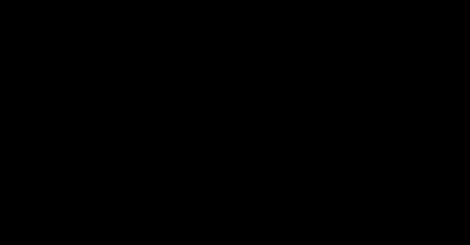
\includegraphics{figure1.pdf}
\caption{Demonstration of the ternary balance scheme showing the
composition of educational attainment by region in Europe, 2016. Data by
Eurostat.}
\end{figure}

\hypertarget{the-challenge-of-unbalanced-compositions}{%
\section{The challenge of unbalanced
compositions}\label{the-challenge-of-unbalanced-compositions}}

While the ternary balance scheme allows for incredibly dense yet clear
visualizations of well-spread-out three-part compositions, the technique
is less informative when used with highly unbalanced data. Figure 2a
shows the regional workforce composition in Europe as of 2016. The map
is almost monochromatic, with the intense magenta signifying a working
population concentrated in the tertiary (services) sector. Regions in
Turkey and Eastern Europe show a somewhat higher concentration of
workers in the primary (production) sector, but overall there is little
variation with regard to the visual reference point, i.e., the
grey-point marking perfectly balanced proportions.

A remedy for analyzing data that show little variation in relation to
some reference point is to adjust the point of reference. Figure 2b yet
again shows the European regional workforce composition, but the data
have been reprojected so that the center of the compositional point
cloud, the average European workforce composition, coincides with the
grey-point of the ternary balance scheme. Consequently, the colors now
show the direction and magnitude of the deviation from that average.
Yellow, cyan, and magenta hues signify a higher-than-average share of
workers in the primary, secondary, and tertiary sectors. The saturation
of the colors encodes the magnitude of that deviation, with perfect grey
marking a region with a workforce composition equal to the European
average, i.e., the new reference point.

The centered ternary balance scheme emerges from an application of a
regular ternary color-coding to transformed (centered) compositional
data. In the following, I explain its construction.

\begin{figure}
\centering
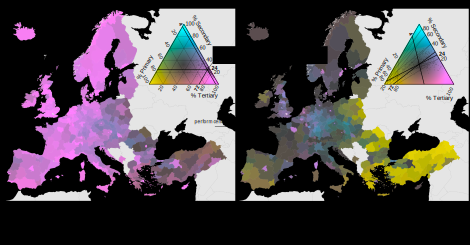
\includegraphics{figure2.pdf}
\caption{Demonstration of the centered ternary balance scheme in
comparison with the non-centered scheme showing the workforce
composition by region in Europe, 2016. Data by Eurostat.}
\end{figure}

\hypertarget{perturbation-and-centering-of-compositional-data}{%
\section{Perturbation and centering of compositional
data}\label{perturbation-and-centering-of-compositional-data}}

Given a series of temperature readings for each day of a year, one may
want to show how each reading compares to the yearly average. By
subtracting the annual average from each data point, a new variable is
created. It represents direction and magnitude of the temperature
deviation from the mean with a reference point at zero. For the domain
of compositional data, a similar transformation goes by the name
perturbation, and it has been proposed as a means of centering
unbalanced observations in a ternary diagram
\citep{VonEynatten2002, PawlowskyGlahn2002}.

When John Aitchison set out the principles of compositional data
analysis \citep{Aitchison1982, Aitchison1986, PawlowskyGlahn2015} he
used ternary diagrams to illustrate the appropriate sample space, a
positive simplex. Compositions are defined as points in the simplex or
equivalently as a vector \(\mathbf{x}\) with positive elements
\(\langle x_1,\ldots,x_D \rangle\) constrained to sum to unity. Just as
the operations of linear algebra are intuitively illustrated in the two
dimensions of the Cartesian plane, coordinates in the ternary diagram
change in reaction to operations on the corresponding simplex, one such
operation being the perturbation of a composition
\(\mathbf{x}=\langle x_1, \ldots, x_D \rangle\) by another
\(\mathbf{y}=\langle y_1, \ldots, y_D \rangle\) defined as
\(\mathbf{x}\oplus \mathbf{y}=\mathcal{C}\langle x_1y_1, \ldots, x_Dy_D \rangle\),
where
\(\mathcal{C}\langle x_1, \ldots, x_D \rangle = \left\langle\frac{x_1}{\sum_i^D x_i},\ldots, \frac{x_D}{\sum_i^D x_i}\right\rangle\)
denotes the closure operation that imposes the unit-sum constraint via
division of each vector element by the sum of all elements. Note that as
a consequence of this definition, the perturbation of any composition
\(\mathbf{y}\) by its inverse
\(\mathbf{y}^{-1}=\langle 1/y_1, \ldots, 1/y_D \rangle\) results in the
neutral element
\(\mathbf{y}\oplus \mathbf{y}^{-1}=\langle 1/D, \ldots, 1/D \rangle\),
which for a three-part composition coincides with the barycenter of a
ternary diagram at \(\langle 1/3, 1/3, 1/3 \rangle\). Thus, perturbation
allows the transformation of coordinates in a ternary diagram such that
an arbitrary composition can be relocated to the center, acting as a
reference point against which all other compositions are compared.
Whenever a compositional data set is perturbed by the inverse of its
compositional mean, the operation is known as centering -- a key
component for the construction of the centered ternary balance scheme as
it allows the color-coding of the deviations from an average, thereby
visualizing structure in surfaces of unbalanced data.

\hypertarget{the-centered-ternary-balance-scheme}{%
\section{The centered ternary balance
scheme}\label{the-centered-ternary-balance-scheme}}

The construction of the centered ternary balance scheme is
straightforward. One needs but two ingredients: 1) the ability to
colorize a ternary composition with the regular ternary balance scheme,
and 2) the ability to perturbate a ternary composition by the inverse of
its compositional mean as proposed by \citet{VonEynatten2002} and
described above. One first performs the centering of the compositional
data set and then colorizes the centered data according to the regular
ternary balance scheme. In the following, I demonstrate how these two
operations resulted in the map of deviations from the average European
workforce composition by region in 2016 (see Figure 2b) and propose
several options for drawing an informative color key.

In 2016 the average European region had 4\% of the workforce situated in
the primary sector, 24\% in the secondary sector, and 72\% in the
tertiary sector. The composition
\(\mathbf{y}=\langle 0.04, 0.24, 0.72 \rangle\) marks the reference
against which all other compositions are to be compared.\footnote{ In
  compositional data analysis, the standard measure of centrality is the
  vector formed by closure of the component-wise geometric means of the
  observed compositions. \citet{VonEynatten2002} advocate for this
  measure to be used when centering data on the ternary diagram and it
  is used here as well. Note, however, that \(\mathbf{y}\) is virtually
  identical to the workforce distribution calculated from the numbers of
  workers in each sector summed across all European regions.} Let
\(\mathbf{x}_j = \langle x_{1j}, x_{2j}, x_{3j} \rangle\) be the
workforce composition of region \(j\) as shown in Figure 3a. For each
region I calculate the perturbation
\(\mathbf{x}'_j = \mathbf{x}_j \oplus \mathbf{y}^{-1}\) shown in Figure
3b. The perturbed compositions are then color-coded according to a
regular ternary balance scheme. The simplest way to achieve this is to
interpret the composition as coordinates in the RGB color space. See,
e.g., \citet{Wang2009} for such an approach. A more flexible method
employed in this paper is described in \citet{Schoeley2017} and is
implemented in the tricolore R package \citep{Schoeley2019a}. Based upon
the CIE-Lch color space -- a transformation of CIE-Luv described in
\citet{Ware2013}, chapter 4 -- the technique allows for different
choices of primary colors and gives the user control over overall
lightness levels and contrast while ensuring that all primary colors
used in the mixing appear roughly equal in lightness and chroma.
Additionally, in the CIE-Lch space, the color dimensions hue, lightness,
and chroma can be manipulated truly independent of each other, a
property not shared by the popular RGB or HSV color spaces
\citep{Zeileis2009}.

The resulting colors show for each composition the direction and
magnitude of deviation from the compositional mean. The hue of the color
encodes which components of a three-part composition are greater than
the average, whereas lightness and saturation indicate the distance of a
composition from the average, which itself is colored grey.

\begin{figure}
\centering
\includegraphics{figure3.pdf}
\caption{Different representations of the color key for the (centered)
ternary balance scheme showing the workforce composition by region in
Europe, 2016. Data by Eurostat.}
\end{figure}

There are multiple options for drawing an informative color key. Simply
plotting the centered compositions in a ternary diagram with a
color-coded background as in Figure 3b -- while correct -- is not very
intuitive, as the transformed compositions cannot be easily
interpreted\footnote{The same situation arises when a logarithmic scale
  is labeled with the logged values as opposed to the values on the
  original scale.}. A better option is to plot the centered data in a
ternary diagram with scale labels indicating the original proportions
(see Figure 3c). Because the centering operation skews the grid lines in
a ternary diagram, centered grid lines have to be plotted
\citep{VonEynatten2002}. This is achieved by perturbing the ternary
coordinates of the grid by the inverse of the center \(\mathbf{y}\). As
the colors encode deviations from the center, the grid lines can
accordingly be labeled with the percent point difference from it. A
third option is to plot the uncentered data in the standard ternary
diagram and perturb the background color surface instead, shifting its
grey-point from the barycenter of the triangle to the location of
\(\mathbf{y}\) (see Figure 3d).

A fourth legend style avoids the ternary diagram altogether and instead
displays the log-ratio-transformed compositions in Cartesian coordinates
(Figure 3e). This style of legend may be preferred by an audience
already familiar with the methods of compositional data analysis as
defined by \citet{Aitchison1982}, who introduced the so-called
(additive) log-ratio transform as a means to analyze compositions in the
unconstrained and familiar space of real numbers. For a three-part
composition \(\mathbf{x}\), the log-ratio transform is defined as
\(\text{alr} \langle x_1, x_2, x_3 \rangle = \langle \log (x_1/x_3), \log (x_2/x_3) \rangle = \langle z_1,z_2 \rangle\)
with inverse
\(\text{alr}^{-1}\langle z_1,z_2 \rangle=\mathcal{C}\langle \exp(z_1), \exp (z_2), 1 \rangle = \langle x_1, x_2, x_3 \rangle\).
The transformation maps the three positive elements of the composition
to an unconstrained pair of coordinates, which may be visualized in a
standard scatterplot. Notably, centering \(\mathbf{x}\) by perturbing
with \(\mathbf{y}^{-1}\) is equivalent to subtracting
\(\text{alr}(\mathbf{y})\) from \(\text{alr}(\mathbf{x})\) and applying
the inverse transform to the result, illustrating the relationship
between perturbation in the simplex and a simple translation of the
origin in real coordinates \citep{Aitchison2005a}.

\hypertarget{discussion}{%
\section{Discussion}\label{discussion}}

With the centered ternary balance scheme -- a straightforward synthesis
of the three-variable balance scheme as described by \citet{Brewer1994}
and the centering operation applied in the context of compositional data
analysis in the ternary diagram \citep{VonEynatten2002} -- I have
proposed a visualization technique capable of showing the divergence of
a three-part compositional surface from its average. The technique can
display the internal variation of a data set, which is narrowly
clustered (as demonstrated in Figure 2). More generally, the centered
scheme may also be employed to show the divergence from \emph{any} point
of reference via perturbation by the inverse of the reference
composition. For example, perturbing the regional distribution of
educational attainment in Figure 1b by the average composition in the
U.S. would yield a map of compositional differences from the U.S.
average. Further, compositional change over time can be visualized by
perturbing each data point at \(t_2\) by the inverse of the
corresponding composition at \(t_1\) \citep{Aitchison2005a} and
colorizing the resulting perturbation using the standard ternary balance
scheme.

Neither the ternary balance scheme nor its centered extension has been
empirically tested regarding the effectiveness of visualizing
compositional data on a surface. However, visualization theory gives
some insight into potential strengths and weaknesses of the technique.
The ternary balance technique uses the visual attribute ``color'' as a
multidimensional encoding for the three parts that make up a ternary
composition, mapping each part of the composition to a separate primary
color channel. Is it possible for a reader of the visualization to
separate the ternary colors into their three primaries, thereby
perceiving the relative magnitude of each compositional part separately?
The answer is no. Color primaries are known to be integral: they are
perceived jointly and are hard to separate \citep{Ware2013}. Therefore,
the ternary balance technique should not be used in situations where it
is essential to precisely identify the relative shares of three
components. However, the scheme can also be interpreted as a
hue-(lightness/chroma) encoding. While hue signifies a qualitative
attribute -- the dominant part(s) of the composition -- lightness and
chroma redundantly encode the distance of a compositional observation
from a reference composition -- a quantitative attribute. Hue and
lightness can be separated to some degree, as illustrated by color names
such as light blue, dark green, and so forth. Interpreting the hues and
lightness components of a map colored with the ternary balance scheme
allows numerous relevant tasks to be performed:

\begin{enumerate}
\def\labelenumi{\arabic{enumi}.}
\tightlist
\item
  \textbf{Identification of regions close to the reference composition.}
  Locate dark and grey regions.
\item
  \textbf{Identification of regions deviating from the reference
  composition.} Locate bright and colorful regions.
\item
  \textbf{Classification of regions deviating from the reference
  composition.} Identify the hue of the region and associate the hue
  with its corresponding part(s) of the composition.
\item
  \textbf{Identification of compositional spatial gradients.} Locate
  color gradients.
\item
  \textbf{Classification of compositional spatial gradients.} Identify
  the starting hue and ending hue of the gradient. Associate the
  starting and ending hues with their corresponding part of the
  composition.
\item
  \textbf{Identification of compositional spatial discontinuities.}
  Locate sudden shifts in hue and lightness.
\item
  \textbf{Classification of compositional spatial discontinuities.}
  Identify the hues at both sides of the discontinuity and associate
  them with the corresponding part of the composition.
\end{enumerate}

None of the above tasks requires the reader to perform the impossible
feat of decomposing a color into its primary constituents. The
identification tasks 1 and 2 can be performed solely by comparing
lightness levels. Identification tasks 4 and 6 require judging the
dissimilarity of neighboring colors. Classification tasks 3, 5, and 7
require the rough matching of two hues. All of these perception and
cognitive tasks can also be found in established visualization
techniques. Therefore I hypothesize that they can also be performed on
the ternary balance scheme. Empirical evidence has to be collected to
support that claim.

Whenever hue is used as a visual encoding, consideration has to be given
to people with impaired color vision. Because the ternary balance scheme
relies on the mixture of three distinct primaries, the resulting space
of possible colors will necessarily contain colors that are
non-discriminable by people with impaired color vision. The most common
form of color-blindness reduces the sensitivity to green light, making
it hard to distinguish colors along the red-green spectrum
\citep{Birch2012}. If the compositional data set does not cover the
whole surface of the ternary legend, then it may be possible to choose
the primary colors such that the data fall outside of the red-green
spectrum.

\begin{figure}
\centering
\includegraphics{figure4.png}
\caption{The tricolore package for the statistical programming language
R implements the centered ternary balance color scheme and provides a
user interface for quickly testing different parametrizations.}
\end{figure}

The technique described in this paper is implemented in the tricolore R
package \citep{Schoeley2019a},\footnote{Development takes place in a
  public repository at \url{https://github.com/jschoeley/tricolore} and
  the authors welcome suggestions and bug reports.} which builds upon
the facilities of the ggtern package \citep{Hamilton2018} to draw
color-coded ternary diagrams. Given a three-column matrix of three-part
compositions, tricolore returns a vector of colors and a suitable color
key. The user may choose between discrete and continuous color scales,
center the color scale around either the geometric mean of the provided
data or an arbitrary reference composition, and experiment with
different values for hue, lightness, chroma, and contrast. An online
tutorial \citep{Schoeley2019b} explains how to use the software to
create color-coded maps like those shown in this paper, and a user
interface (see Figure 4) helps with picking suitable parameters for the
color scale. Thus far the software has been used in publications to map
regional deviations from the average European age composition
\citep{Kashnitsky2018, Schoeley2019}, disparities in regional education
attainment in India and Nigeria \citep{Graetz2019}, the cause of death
distribution by period, age, and region in Mexico
\citep{Kashnitsky2019}, and Vienna's district population mix by region
of origin \citep{StadtWien2019}. I hope that tricolore continues to
encourage people to experiment with this novel visualization technique
-- three-part compositions are plenty, and surfaces, whether defined by
longitude and latitude or by period and age, provide ample room to find
exciting variation in the data.

\hypertarget{acknowledgments}{%
\section{Acknowledgments}\label{acknowledgments}}

My thanks go to the three reviewers who generously contributed their
time and expertise. I would also like to thank Marie-Pier Bergeron
Boucher and Jim Oeppen for their input regarding the analysis of
compositional data and Ilya Kashnitsky, who inspired me to write this
paper.

%--- Print references --------------------------------------------------

\newpage

\addcontentsline{toc}{section}{\numberline{}References}

\bibliography{references.bib}

%--- Print appendix ----------------------------------------------------


%--- End document ------------------------------------------------------

\cleardoublepage

\end{document}
